\documentclass[../main.tex]{subfiles}
\graphicspath{{\subfix{../images/}}}
\begin{document}
\section*{Term 2 Week 3}
\begin{enumerate}
    \item 
    The first polynomial implies that \(st=s\), since the polynomial can be factorised into the form \((x-s)(x-t)\), therefore \(t=1\).\\

    Since \(x^2+tx+r\) has 5 as a root, by the Factor Theorem we know that \(5^2+5t+r=0\), and since \(t=1\) we know that \(r=-30\).\\

    Returning to the first polynomial, \(x^2-30x+s\) has 1 as a root (the value of \textit{t}), so again by the Factor Theorem, we know that \(1^2-30+s=0\), giving \(s=29\).\\
    
    \item 
    Isabella's sum is the \(ab^{th}\) triangle number, given by \(\frac{ab(ab+1}{2}\).\\

    Vidur's sum comprises rows that are increasing multiples of the \(b^{th}\) triangle number:\\
    \(1(\frac{b(b+1)}{2})+2(\frac{b(b+1)}{2})+...+a(\frac{b(b+1)}{2})\)\\
    \((1+2+...+a)(\frac{b(b+1)}{2})\)\\
    \(\frac{a(a+1)}{2} \times \frac{b(b+1)}{2}\)\\

    The difference is:\\
    \(\frac{ab(ab+1}{2}-\frac{a(a+1)}{2} \times \frac{b(b+1)}{2}=1200\)\\
    
    \(\frac{2ab(ab+1)-(a+1)(b+1)}{4}=1200\)\\
    
    \(\frac{ab(2ab+2-ab-a-b-1)}{4}=1200\)\\

    \(\frac{ab(ab-a-b+1)}{4}=1200\)\\

    \(\frac{ab(a-1)(b-1)}{4}=1200\)\\

    \(ab(a-1)(b-1)=4800\)\\

    \(a(a-1)\times b(b-1)=4800\)\\

    Arbitrarily assume that \(b\leq a\), which means \(b(b-1) \leq a(a-1)\). This means that \(b(b-1) < 70\) (because it must be less than the square root of 4800), therefore \(b \leq 8\).\\

    If \(b=7\) or \(b=8\), then \(b(b-1)\) has a factor of 7, which 4800 does not, therefore they cannot be the solution and \(b \leq 6\).\\

    If \(b=6, b(b-1)=30\), which is a factor of 4800. This means \(a(a-1)=160\). However, this has no solution so \textit{b} cannot be 6.\\

    If \(b=5, b(b-1)=20\), which is also a factor 4800. This means \(a(a-1)=240\). Solving, \(a=16\).\\

    This means that \(a+b=5+16=21\)\\
    
    \item 
    Add \textit{x} to both sides:\\
    \(f(x)+x=2x+\frac{1}{2x+\frac{1}{2x+\frac{1}{2x+...}}}\)\\
    
    Comparing the two right-hand sides, we see that the RHS of the second equation is the same as the denominator of the first. Substituting the second equation into the first:\\
    \(f(x)=x+\frac{1}{f(x)+x}\)\\

    Subtracting \textit{x} from both sides:\\
    \(f(x)-x=\frac{1}{f(x)+x}\)\\

    Cross-multiplying:\\
    \([f(x)-x][f(x)+x]=1\)\\
    \([f(x)]^2-x^2=1\)\\

    Differentiating (notice that we use the Chain Rule), we get:\\
    \(2f(x)\times f'(x)-2x=0\)\\
    
    Simplifying and rearranging:\\
    \(f(x).f'(x)-x=0\)\\
    \(f(x).f'(x)=x\)\\

    Now if we substitute in \(x=99\) as per the original question:\\
    \(f(99).f'(99)=99\)\\

    \item 
    Forming a triangle from a bottom vertex of the larger triangle to the centre of the triangle, we get a 30-60-90 triangle with sides in the ratio \(1:2:\sqrt{3}\).
    \begin{figure}[H]
        \centering
        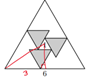
\includegraphics[width=0.25\linewidth]{images/t2w3q4_a1.png}
    \end{figure}
    This triangle is \(\sqrt{3}\) times larger than the standard ratio triangle, so the side lengths are:
    \begin{figure}[H]
        \centering
        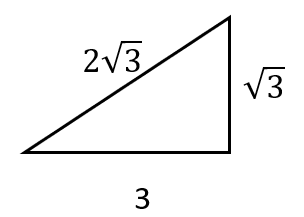
\includegraphics[width=0.2\linewidth]{images/t2w3q4_a2.png}
    \end{figure}
    This means that the distance from the centre of the base of the larger triangle to the centre is \(\sqrt{3}\).\\
    We can now calculate the distance from the centre of the base of the smallest triangle to the centre of the larger triangle, as it has lengths exactly 6 times smaller.\\
    This gives us:
    \begin{figure}[H]
        \centering
        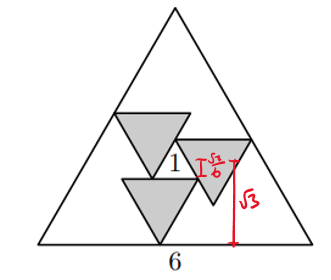
\includegraphics[width=0.25\linewidth]{images/t2w3q4_a3.png}
    \end{figure}
    Now we find the height of each of the grey triangles.
    \begin{figure}[H]
        \centering
        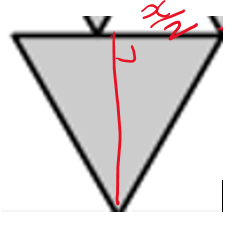
\includegraphics[width=0.25\linewidth]{images/t2w3q4_a4.png}
    \end{figure}
    This is another 30-60-90 triangle, therefore the height of the grey triangle is \(\frac{\sqrt{3}}{2}x\).\\
    We now have:
    \begin{figure}[H]
        \centering
        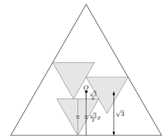
\includegraphics[width=0.3\linewidth]{images/t2w3q4_a5.png}
    \end{figure}
    \(\sqrt{3}-\frac{\sqrt{3}}{6}=\frac{\sqrt{3}}{2}x\)\\
    \(\frac{5\sqrt{3}}{6}=\frac{\sqrt{3}}{2}x\)\\
    \(x=\frac{5}{3}\)\\
    
    \item 
    If \(n^2-3000\) is a perfect square, then \((-n)^2-3000\) is also a perfect square. Therefore, the sum is zero.
    
\end{enumerate}

\end{document}